\let\negmedspace\undefined
\let\negthickspace\undefined
\documentclass[journal]{IEEEtran}
\usepackage[a5paper, margin=10mm, onecolumn]{geometry}
%\usepackage{lmodern} % Ensure lmodern is loaded for pdflatex
\usepackage{tfrupee} % Include tfrupee package

\setlength{\headheight}{1cm} % Set the height of the header box
\setlength{\headsep}{0mm}     % Set the distance between the header box and the top of the text

\usepackage{gvv-book}
\usepackage{gvv}
\usepackage{cite}
\usepackage{amsmath,amssymb,amsfonts,amsthm}
\usepackage{amsmath}
\usepackage{algorithmic}
\usepackage{graphicx}
\usepackage{textcomp}
\usepackage{xcolor}
\usepackage{txfonts}
\usepackage{listings}
\usepackage{enumitem}
\usepackage{mathtools}
\usepackage{gensymb}
\usepackage{comment}
\usepackage[breaklinks=true]{hyperref}
\usepackage{tkz-euclide} 
\usepackage{listings}
% \usepackage{gvv}                                        
\def\inputGnumericTable{}                                 
\usepackage[latin1]{inputenc}                                
\usepackage{color}                                            
\usepackage{array}                                            
\usepackage{longtable}                                       
\usepackage{calc}                                             
\usepackage{multirow}                                         
\usepackage{hhline}                                           
\usepackage{ifthen}                                           
\usepackage{lscape}
\usepackage{circuitikz}
\tikzstyle{block} = [rectangle, draw, fill=blue!20, 
    text width=4em, text centered, rounded corners, minimum height=3em]
\tikzstyle{sum} = [draw, fill=blue!10, circle, minimum size=1cm, node distance=1.5cm]
\tikzstyle{input} = [coordinate]
\tikzstyle{output} = [coordinate]


\begin{document}

\bibliographystyle{IEEEtran}
\vspace{3cm}

\title{4.8.14}
\author{AI25BTECH11018-Hemanth Reddy}
 \maketitle
% \newpage
% \bigskip
{\let\newpage\relax\maketitle}

\renewcommand{\thefigure}{\theenumi}
\renewcommand{\thetable}{\theenumi}
\setlength{\intextsep}{10pt} % Space between text and floats


\numberwithin{equation}{enumi}
\numberwithin{figure}{enumi}
\renewcommand{\thetable}{\theenumi}

\textbf{Question:}\\

Let $\vec{P} (3,2,6)$ be a point in space and $\vec{Q}$ be a point on the line
$ \vec{r} = (\hat{i} - \hat{j} + 2\hat{k}) + \mu(-3\hat{i} + \hat{j} + 5\hat{k}). $
Then the value of $\mu$ for which the vector $\overrightarrow{PQ}$ is parallel to the plane $x - 4y + 3z = 1$ is 


\textbf{Solution:}\\


\begin{align}
   \text{ The position vector of point }  \vec{P} \text{ is }
 \myvec{ 3 \\ 2\\ 6 } 
\end{align}

Point $\vec{Q}$ lies on line $\vec{r}$ .So

\begin{align}
   \text{ The position vector of point }  \vec{Q} \text{ is }
 \myvec{ 1-3\mu\\ -1+\mu \\ 2+5\mu } 
\end{align}

\begin{align}
    \overrightarrow{PQ} = \vec{Q} -\vec{P} = \myvec{ 1-3\mu-3\\ -1+\mu -2\\ 2+5\mu -6} = \myvec{ -2-3\mu\\ -3+\mu \\ -4+5\mu } 
\end{align}
Equation of plane is $x - 4y + 3z = 1$ 
\begin{align}
    \text{ Normal of plane is} \quad \vec{n} =\myvec{ 1 \\ -4\\ 3 } 
\end{align}

$\overrightarrow{PQ}$ is parallel to the plane ,So $\vec{n}^{T}(\vec{PQ})=0$

\begin{align}
   \vec{n}^{T}(\vec{PQ})= \myvec{ 1 & -4 & 3 } \myvec{ -2-3\mu\\ -3+\mu \\ -4+5\mu } =0
\end{align}

\begin{align}
    -2-3\mu+12-4\mu-12+15\mu=0\\
    -2+8\mu=0\\
    \mu=\frac{1}{4}
\end{align}


\begin{figure}
    \centering
    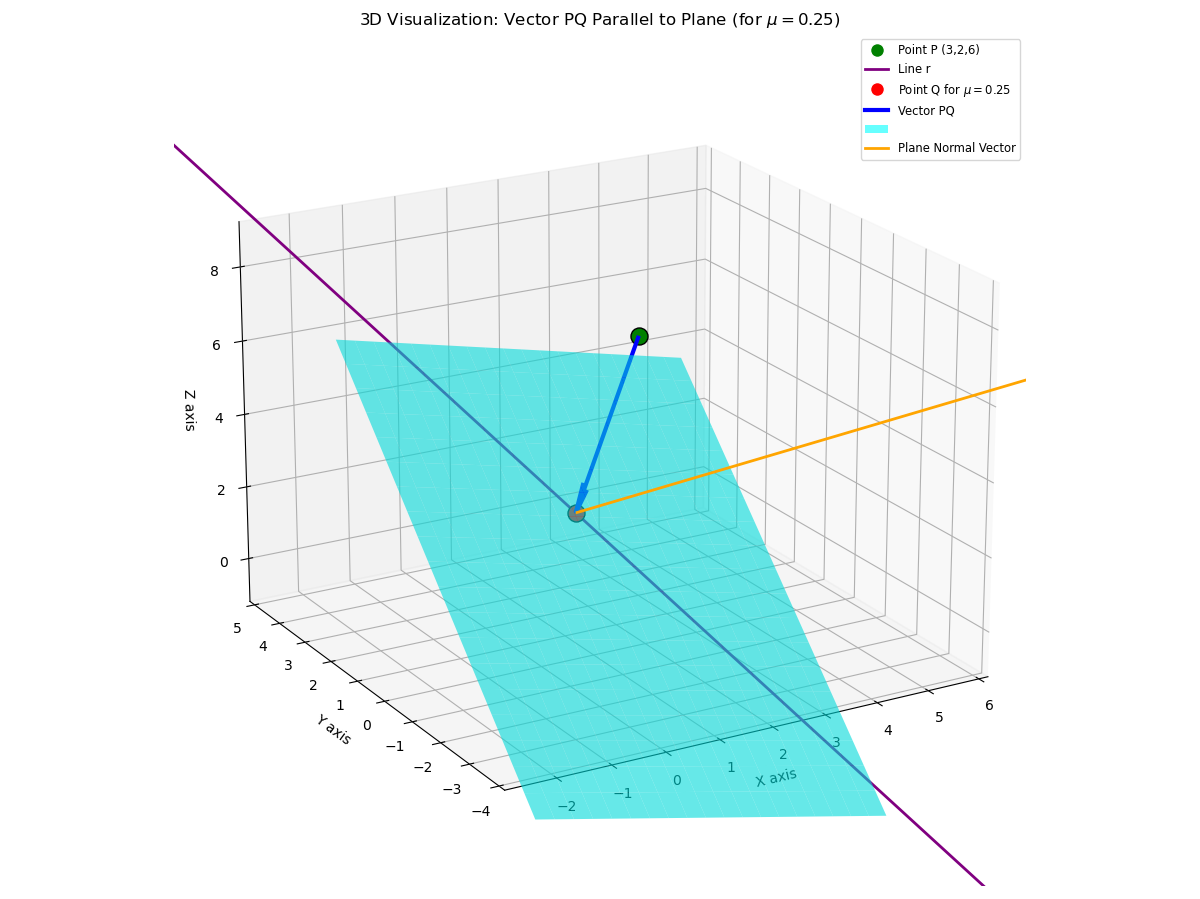
\includegraphics[width=1\linewidth]{figs/Plane1.png}
    \caption{}
    \label{fig:placeholder}
\end{figure}



\end{document}